\section{Outils et technologies}
\label{sec.tech}

La création d'un système aussi sophistiqué que le nôtre est une tâche assez complexe.
Elle comporte plusieurs étapes dont certaines nécessite d'entraîner des réseaux de neurones 
ou de faire appel à des réseaux de neurones pré-entraînés par le biais d'\glspl{abb.api}.
Pour faciliter certaines de ces étapes, nous avons exploité plusieurs outils et technologies open-source.
Cette section est consacrée à la présentation de ces derniers.

\subsection{Python}
\label{subsec.python}

\begin{wrapfigure}{r}[-10pt]{3cm}
    \vspace*{-\topsep}
    \centering
    
\includegraphics[width=3cm]{assets/images/python-logo.png}
\end{wrapfigure}
Python est un langage de programmation open-source interprété, orienté objet et multiparadigme.
Introduit 1991 par Guido van Rossum~\cite{Python_2022},
Python est aujourd'hui l'un des langages de programmation les plus populaires au monde.
Le~\cite{StackOverflowSurvey2022} l'a classé comme la 4\ieme{} technologie la plus populaire au monde (48.07\%)
et la 6\ieme{} technologie la plus aimée (67.34\%).
La documentation officielle de Python le décrit comme suit :

\begin{quote}
    ``Python est un langage de programmation puissant et facile à apprendre. 
    Il dispose de structures de données de haut niveau 
    et permet une approche simple, mais efficace de la programmation orientée objet. 
    Parce que sa syntaxe est élégante, que son typage est dynamique et qu'il est interprété, 
    Python est un langage idéal pour l'écriture de scripts 
    et le développement rapide d'applications dans de nombreux domaines et sur la plupart des plateformes.''
\end{quote}
\begin{flushright}
    --- \barecite{py_tut}
\end{flushright}

La popularité de Python fait qu'il y a une grande communauté de développeurs qui contribuent à son écosystème.
En effet, \href{https://pypi.or}{le répoertoire officiel de Python} contient plus de 450 000 packages.
Tous les programmes écrits dans le cadre de ce projet sont écrits en Python.

\subsection{Jupyter}
\label{subsec.jupyter}

\begin{wrapfigure}{r}[-10pt]{3cm}
    \vspace*{-\topsep}
    \begin{flushright}
        
\includegraphics[width=3cm]{assets/images/jupyter.png}
    \end{flushright}
\end{wrapfigure}
Jupyter est un environnement d'exécution interactif pour Python (et plusieurs autres langages).
Il permet de créer des documents appelés ``notebooks'' qui combine le code exécutable avec une documentation textuelle.
Cela est réalisé en divisant le document en unités appelées des ``cellules''.
Une cellule est associée à un langage qui peut-être écrit dedans.
Si ce langage est un langage de programmation (Python, R ou Julia), la cellule est exécutable.
Si ce langage est Markdown, elle ne l'est pas.


\subsection{Google Colaboratory, Kaggle et Paperspace Gradient}
\label{subsec.colab}

\begin{wrapfigure}{r}[-15pt]{3cm}
    \vspace*{-\topsep}
    \begin{flushright}
        
\includegraphics[width=3cm]{assets/images/colab.png}
    \end{flushright}
\end{wrapfigure}
Colaboratory est un service fourni par Google.
Il donne à ses utilisateurs l'accès à un environnement d'exécution Jupyter hébergé sur le cloud.
Il est possible d'y créer et d'y exécuter des notebooks sans installation ni configuration.
Il offre également (et gratuitement) le choix entre les exécuter sur un CPU ou un GPU.
La machine virtuelle qui héberge cet environnement est réinitialisée après 12 h.
Cette limite peut être étendue en utilisant un compte payant.

\begin{wrapfigure}{r}[-10pt]{3cm}
    \vspace*{-\topsep}
    \begin{flushright}
        
\includegraphics[width=3cm]{assets/images/Kaggle_logo.png}
    \end{flushright}
\end{wrapfigure}
Kaggle est une plateforme en ligne qui permet d'organiser des compétitions en data science.
Dans ce cadre, elle donne accès à un environnement similaire à celui trouver sur Google Colaboratory.
Les GPU qu'elle offre ont 16 Go de mémoire.
Le temps de calcul sur Kaggle est limité à 30 heures par semaine.


\begin{wrapfigure}{r}[-10pt]{3cm}
    \vspace*{-\topsep}
    \begin{flushright}
        
\includegraphics[width=2cm]{assets/images/paperspace.png}
    \end{flushright}
\end{wrapfigure}
Paperspace est une plateforme du calcul cloud dédié au \gls{ml} et à l'intelligence artificielle.
Elle permet de créer des machines virtuelles avec des configurations personnalisées.
Paperspace possède une grande variété d'architectures matérielles.
Des CPU et des GPU y sont disponibles, mais aussi des TPU et des IPU.
Il est possible de personnaliser le nombre de CPU, GPU, TPU et IPU à inclure dans une  machine,
ainsi que le type et les caractéristiques des CPU et GPU.

Gradient est un service offert par Paperspace.
Similairement à Google Colaboratory et Kaggle, il permet d'accéder à un environnement Jupyter hébergé sur le cloud.
Cependant, il offre plus de flexibilité que ces derniers.
Il permet de personnaliser d'une manière similaire aux machines virtuelles de Paperspace.
\ \\

\subsection{Anaconda}
\label{subsec.anaconda}

\begin{wrapfigure}{r}[-25pt]{2cm}
    \vspace*{-\topsep}
    \begin{flushright}
        
\includegraphics[width=2cm]{assets/images/anaconda.png}
    \end{flushright}
\end{wrapfigure}
Anaconda est une distribution logicielle open-source qui regroupe 
Python, R et une multitude de leurs packages consacrés au calcul scientifique et aux data science.
Anaconda permet de créer des environnements virtuels pour Python pour isoler les dépendances entre les projets.
Chaque environnement possède sa propre installation de Python et de ses packages.
Un gestionnaire de packages appelé ``\texttt{conda}'' est fourni comme alternative à \texttt{pip}.


\subsection{CUDA}
\label{subsec.cuda}

\begin{wrapfigure}{r}[-20pt]{2cm}
    \vspace*{-\topsep}
    \begin{flushright}
        
\includegraphics[width=2cm]{assets/images/nvidia.png}
    \end{flushright}
\end{wrapfigure}
CUDA est une technologie de calcul parallèle développée par NVIDIA.
Elle permet d'utiliser les GPU de NVIDIA pour accélérer les calculs parallélisables.
CUDA est programmable en C++.
Cependant, il existe des bibliothèques qui permettent de l'utiliser avec d'autres langages (y compris Python).


\subsection{PyTorch}
\label{subsec.pytorch}

\begin{wrapfigure}{r}[-10pt]{3cm}
    \vspace*{-\topsep}
    \begin{flushright}
        
\includegraphics[width=2cm]{assets/images/torch.png}
    \end{flushright}
\end{wrapfigure}
PyTorch est une bibliothèque open-source de \gls{dl} pour Python.
Elle permet de créer et d'entraîner rapidement et facilement des réseaux de neurones.
Elle est développée par Facebook AI, mais elle fait rejoint la fondation Linux en 2022.

PyTorch possède plusieurs modules.
Les plus importants sont :
\begin{itemize}
    \item \verb|torch.Tensor| : 
    ce module fournit une implémentation du tenseur,
    un tableau multidimensionnel qui peut être manipulé mathématiquement 
    d'une façon qui généralise les scalaires, les vecteurs et les matrices.
    \item \verb|torch.nn| : 
    ce module contient une implémentation des réseaux de neurones.
    La classe la plus importante dans ce module est \verb|torch.nn.Module|.
    Il s'agit d'une classe abstraite qui doit être héritée pour créer un réseau de neurones.
    Des implémentations pour les architectures les plus courantes sont fournies dans ce module
    (\gls{cnn}, \gls{rnn}, transformeur, etc.).
    \item \verb|torch.optim| : 
    ce module offre un ensemble d'algorithmes d'optimisation.
    \item \verb|torch.autograd| : 
    ce module fournit une implémentation de la dérivation automatique (\foreignlanguage{english}{backward}).
    Il permet de calculer les gradients des paramètres en construisant un graphe de calcul 
    puis en le traversant pour évaluer les dérivées.
\end{itemize}
Toutes les opérations de PyTorch peuvent être exécutées sur un GPU en utilisant CUDA.
Cela rend très rapide l'entraînement des réseaux de neurones.

L'écosystème de PyTorch est très riche.
Plusieurs packages sont construits là-dessus par la communauté ainsi que par l'équipe de PyTorch.
Parmi les packages \verb|torchtext| et \verb|torchdata| nous sont les plus utiles.
Le premier nous offre des objets utiles pour le traitement de texte en langage naturel
(tokeniseurs, jeux de données populaires, modèles de langage, etc.).
Le second implémente les fonctionnalités de manipulation de données.
Les deux classes les plus importantes dans ce module sont \verb|torchdata.Dataset| et \verb|torchdata.DataLoader|.

\subsection{\foreignlanguage{english}{Lightning}}
\label{subsec.lightning}

\begin{wrapfigure}{r}[-15pt]{2cm}
    \vspace*{-\topsep}
    \begin{flushright}
        
\includegraphics[width=2cm]{assets/images/lightning.png}
    \end{flushright}
\end{wrapfigure}
\foreignlanguage{english}{Lightning.AI} est une plateforme pour créer, entraîner et déployer des modèles de \gls{dl}.
La bibliothèque \verb|lightning| distribuée contient 3 packages (voir Figure~\ref{fig.lightning-structure}) :
\begin{itemize}
    \item \verb|lightning.pytorch| 
    \item \verb|lightning.fabric|
    \item \verb|lightning.applications|
\end{itemize}

\begin{figure}[hbt]
    \begin{center}
        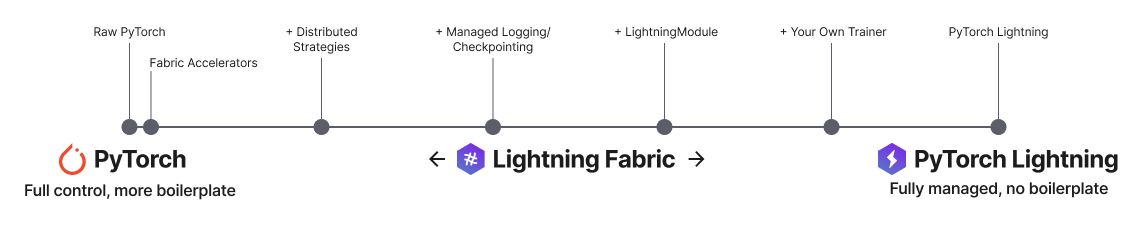
\includegraphics[width=\linewidth]{assets/images/lightning-strcture.png}
    \end{center}
    \cprotect\caption[Composantes de la bibliothèque \verb|lightning|.]%
    {Composantes de la bibliothèque \verb|lightning|~\cite{Falcon_PyTorch_Lightning_2019}.}
    \label{fig.lightning-structure}
\end{figure}

\verb|lightning.pytorch| (aussi appelé \verb|pytorch-lightning|) est le seul que nous avons utilisé.
Il permet d'étendre PyTorch pour faciliter la création et l'entraînement des modèles.
Les fonctionnalités qu'il offre incluent les rappels de fonctions et la journalisation.

\foreignlanguage{english}{Lightning.AI} distribue un quatrième package en dehors de la bibliothèque \verb|lightning| :
\verb|torchmetrics|.
Ce dernier implémente plus de 90 métriques d'évaluation, dont l'exactitude et le score \gls{bleu}.
Nous avons fait usage de ce package pour calculer ces métriques.

\subsection{\foreignlanguage{english}{Weights \& Biases}}
\label{subsec.wandb}

\foreignlanguage{english}{Weights \& Biases} est une plateforme de \gls{abb.mlops}.
Son but est de faciliter le processus de développement de journalisation des expériences,
de gestion des versions de jeux de données et de collaboration entre les membres d'une équipe.
\begin{wrapfigure}{r}[-15pt]{2cm}
    % \vspace*{-\topsep}
    \begin{flushright}
        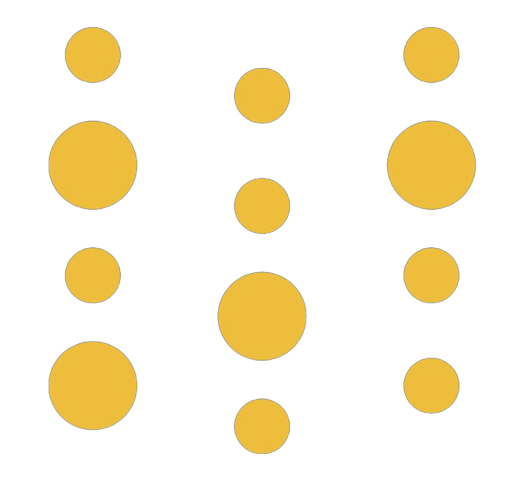
\includegraphics[width=2cm]{assets/images/wandb.png}
    \end{flushright}
\end{wrapfigure}

l'\gls{abb.api} de \foreignlanguage{english}{Weights \& Biases} est accessible via un module Python \verb|wandb|
ou via une interface en ligne de commande du même nom.
Elle offre la possibilité de journaliser les métriques d'évaluation, les hyperparamètres, les graphes de calcul, etc.
Elle est intégrée avec \verb|lightning| à travers la classe \verb|lightning.pytorch.loggers.WandbLogger|.

\subsection{\foreignlanguage{english}{Hugging Face}}
\label{subsec.huggingface}

\foreignlanguage{english}{Hugging Face} est une entreprise qui se spécialise en intelligence artificielle.
Elle distribue gratuitement plusieurs bibliothèques open-source et des modèles pré-entraînés.
\begin{wrapfigure}{r}[-15pt]{2cm}
    \vspace*{-\topsep}
    \begin{flushright}
        
\includegraphics[width=2cm]{assets/images/huggingface.png}
    \end{flushright}
\end{wrapfigure}

Parmi ces bibliothèques, nous avons utilisé \verb|tokenizers| qui permet de créer des tokeniseurs
et \verb|evaluate| qui implémente plusieurs métriques d'évaluation (dont la perplexité).
Nous l'avons utilisé plutôt que \verb|torchmetrics|, 
car elle permet d'utiliser les modèles pré-entraînés dans \foreignlanguage{english}{Hugging Face Hub}.

\subsection{\foreignlanguage{english}{Open AI}}
\label{subsec.openai}

\begin{wrapfigure}{r}[-20pt]{2cm}
    \vspace*{-\topsep}
    \begin{flushright}
        
\includegraphics[width=2cm]{assets/images/openai.png}
    \end{flushright}
\end{wrapfigure}
\foreignlanguage{english}{Open AI} est une entreprise de recherche en intelligence artificielle.
C'est cette entreprise qui a créé les modèles \gls{gpt} et Whisper discutés dans le chapitre~\ref{chap.mt-and-asr}.

Nous avons fait appel à l'\gls{abb.api} de \foreignlanguage{english}{Open AI} pour utiliser chatGPT,
une version de \gls{gpt}-3 qui est entraînée sur des conversations.
Nous l'avons utilisé pour générer les erreurs synthétiques.
Nous avons également utilisé Whisper pour la transcription des vidéos collectées,
mais nous l'avons utilisé localement, car il est open-source.

\subsection{Pynecone}
\label{subsec.pynecone}

% \begin{wrapfigure}{r}[-30pt]{2cm}
%     \vspace*{-\topsep}
%     \begin{flushright}
%         
\includegraphics[width=2cm]{assets/images/pynecone.png}
%     \end{flushright}
% \end{wrapfigure}

Pynecone est une bibliothèque qui permet de développer des sites web entièrement en Python
(sans besoin d'écrire du code HTML, CSS ou JavaScript).
Nous l'avons utilisé pour créer une interface web pour le modèle de correction d'erreurs.